% Created by tikzDevice version 0.12.3 on 2020-01-31 13:10:19
% !TEX encoding = UTF-8 Unicode
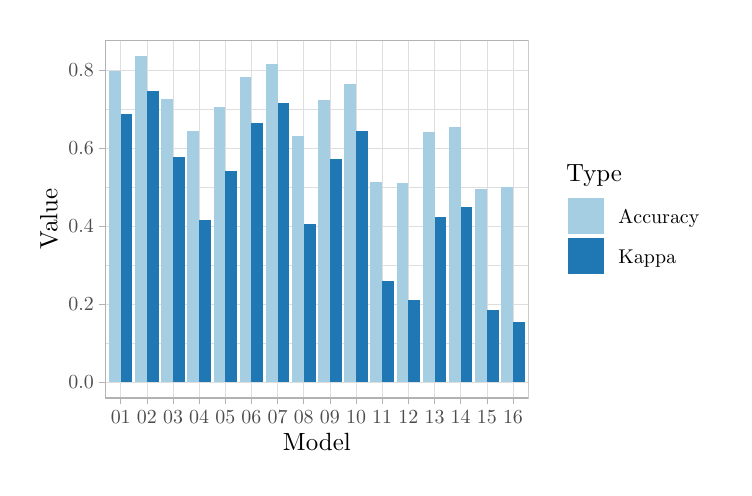
\begin{tikzpicture}[x=1pt,y=1pt]
\definecolor{fillColor}{RGB}{255,255,255}
\path[use as bounding box,fill=fillColor,fill opacity=0.00] (0,0) rectangle (251.50,158.99);
\begin{scope}
\path[clip] (  0.00,  0.00) rectangle (251.50,158.99);
\definecolor{drawColor}{RGB}{255,255,255}
\definecolor{fillColor}{RGB}{255,255,255}

\path[draw=drawColor,line width= 0.5pt,line join=round,line cap=round,fill=fillColor] (  0.00,  0.00) rectangle (251.50,158.99);
\end{scope}
\begin{scope}
\path[clip] ( 27.95, 25.11) rectangle (181.03,154.49);
\definecolor{fillColor}{RGB}{255,255,255}

\path[fill=fillColor] ( 27.95, 25.11) rectangle (181.03,154.49);
\definecolor{drawColor}{gray}{0.87}

\path[draw=drawColor,line width= 0.1pt,line join=round] ( 27.95, 45.08) --
	(181.03, 45.08);

\path[draw=drawColor,line width= 0.1pt,line join=round] ( 27.95, 73.26) --
	(181.03, 73.26);

\path[draw=drawColor,line width= 0.1pt,line join=round] ( 27.95,101.43) --
	(181.03,101.43);

\path[draw=drawColor,line width= 0.1pt,line join=round] ( 27.95,129.61) --
	(181.03,129.61);

\path[draw=drawColor,line width= 0.2pt,line join=round] ( 27.95, 30.99) --
	(181.03, 30.99);

\path[draw=drawColor,line width= 0.2pt,line join=round] ( 27.95, 59.17) --
	(181.03, 59.17);

\path[draw=drawColor,line width= 0.2pt,line join=round] ( 27.95, 87.34) --
	(181.03, 87.34);

\path[draw=drawColor,line width= 0.2pt,line join=round] ( 27.95,115.52) --
	(181.03,115.52);

\path[draw=drawColor,line width= 0.2pt,line join=round] ( 27.95,143.70) --
	(181.03,143.70);

\path[draw=drawColor,line width= 0.2pt,line join=round] ( 33.62, 25.11) --
	( 33.62,154.49);

\path[draw=drawColor,line width= 0.2pt,line join=round] ( 43.07, 25.11) --
	( 43.07,154.49);

\path[draw=drawColor,line width= 0.2pt,line join=round] ( 52.52, 25.11) --
	( 52.52,154.49);

\path[draw=drawColor,line width= 0.2pt,line join=round] ( 61.97, 25.11) --
	( 61.97,154.49);

\path[draw=drawColor,line width= 0.2pt,line join=round] ( 71.41, 25.11) --
	( 71.41,154.49);

\path[draw=drawColor,line width= 0.2pt,line join=round] ( 80.86, 25.11) --
	( 80.86,154.49);

\path[draw=drawColor,line width= 0.2pt,line join=round] ( 90.31, 25.11) --
	( 90.31,154.49);

\path[draw=drawColor,line width= 0.2pt,line join=round] ( 99.76, 25.11) --
	( 99.76,154.49);

\path[draw=drawColor,line width= 0.2pt,line join=round] (109.21, 25.11) --
	(109.21,154.49);

\path[draw=drawColor,line width= 0.2pt,line join=round] (118.66, 25.11) --
	(118.66,154.49);

\path[draw=drawColor,line width= 0.2pt,line join=round] (128.11, 25.11) --
	(128.11,154.49);

\path[draw=drawColor,line width= 0.2pt,line join=round] (137.56, 25.11) --
	(137.56,154.49);

\path[draw=drawColor,line width= 0.2pt,line join=round] (147.01, 25.11) --
	(147.01,154.49);

\path[draw=drawColor,line width= 0.2pt,line join=round] (156.46, 25.11) --
	(156.46,154.49);

\path[draw=drawColor,line width= 0.2pt,line join=round] (165.91, 25.11) --
	(165.91,154.49);

\path[draw=drawColor,line width= 0.2pt,line join=round] (175.36, 25.11) --
	(175.36,154.49);
\definecolor{fillColor}{RGB}{31,120,180}

\path[fill=fillColor] ( 33.62, 30.99) rectangle ( 37.87,127.84);
\definecolor{fillColor}{RGB}{166,206,227}

\path[fill=fillColor] ( 29.36, 30.99) rectangle ( 33.62,143.47);
\definecolor{fillColor}{RGB}{31,120,180}

\path[fill=fillColor] ( 43.07, 30.99) rectangle ( 47.32,135.96);
\definecolor{fillColor}{RGB}{166,206,227}

\path[fill=fillColor] ( 38.81, 30.99) rectangle ( 43.07,148.61);
\definecolor{fillColor}{RGB}{31,120,180}

\path[fill=fillColor] ( 52.52, 30.99) rectangle ( 56.77,112.11);
\definecolor{fillColor}{RGB}{166,206,227}

\path[fill=fillColor] ( 48.26, 30.99) rectangle ( 52.52,133.30);
\definecolor{fillColor}{RGB}{31,120,180}

\path[fill=fillColor] ( 61.97, 30.99) rectangle ( 66.22, 89.60);
\definecolor{fillColor}{RGB}{166,206,227}

\path[fill=fillColor] ( 57.71, 30.99) rectangle ( 61.97,121.49);
\definecolor{fillColor}{RGB}{31,120,180}

\path[fill=fillColor] ( 71.41, 30.99) rectangle ( 75.67,107.30);
\definecolor{fillColor}{RGB}{166,206,227}

\path[fill=fillColor] ( 67.16, 30.99) rectangle ( 71.41,130.25);
\definecolor{fillColor}{RGB}{31,120,180}

\path[fill=fillColor] ( 80.86, 30.99) rectangle ( 85.12,124.56);
\definecolor{fillColor}{RGB}{166,206,227}

\path[fill=fillColor] ( 76.61, 30.99) rectangle ( 80.86,141.06);
\definecolor{fillColor}{RGB}{31,120,180}

\path[fill=fillColor] ( 90.31, 30.99) rectangle ( 94.57,131.67);
\definecolor{fillColor}{RGB}{166,206,227}

\path[fill=fillColor] ( 86.06, 30.99) rectangle ( 90.31,145.70);
\definecolor{fillColor}{RGB}{31,120,180}

\path[fill=fillColor] ( 99.76, 30.99) rectangle (104.02, 87.96);
\definecolor{fillColor}{RGB}{166,206,227}

\path[fill=fillColor] ( 95.51, 30.99) rectangle ( 99.76,119.92);
\definecolor{fillColor}{RGB}{31,120,180}

\path[fill=fillColor] (109.21, 30.99) rectangle (113.47,111.71);
\definecolor{fillColor}{RGB}{166,206,227}

\path[fill=fillColor] (104.96, 30.99) rectangle (109.21,132.84);
\definecolor{fillColor}{RGB}{31,120,180}

\path[fill=fillColor] (118.66, 30.99) rectangle (122.92,121.59);
\definecolor{fillColor}{RGB}{166,206,227}

\path[fill=fillColor] (114.41, 30.99) rectangle (118.66,138.73);
\definecolor{fillColor}{RGB}{31,120,180}

\path[fill=fillColor] (128.11, 30.99) rectangle (132.37, 67.43);
\definecolor{fillColor}{RGB}{166,206,227}

\path[fill=fillColor] (123.86, 30.99) rectangle (128.11,103.07);
\definecolor{fillColor}{RGB}{31,120,180}

\path[fill=fillColor] (137.56, 30.99) rectangle (141.82, 60.47);
\definecolor{fillColor}{RGB}{166,206,227}

\path[fill=fillColor] (133.31, 30.99) rectangle (137.56,102.90);
\definecolor{fillColor}{RGB}{31,120,180}

\path[fill=fillColor] (147.01, 30.99) rectangle (151.27, 90.64);
\definecolor{fillColor}{RGB}{166,206,227}

\path[fill=fillColor] (142.76, 30.99) rectangle (147.01,121.16);
\definecolor{fillColor}{RGB}{31,120,180}

\path[fill=fillColor] (156.46, 30.99) rectangle (160.72, 94.26);
\definecolor{fillColor}{RGB}{166,206,227}

\path[fill=fillColor] (152.21, 30.99) rectangle (156.46,123.21);
\definecolor{fillColor}{RGB}{31,120,180}

\path[fill=fillColor] (165.91, 30.99) rectangle (170.17, 57.06);
\definecolor{fillColor}{RGB}{166,206,227}

\path[fill=fillColor] (161.66, 30.99) rectangle (165.91,100.60);
\definecolor{fillColor}{RGB}{31,120,180}

\path[fill=fillColor] (175.36, 30.99) rectangle (179.62, 52.53);
\definecolor{fillColor}{RGB}{166,206,227}

\path[fill=fillColor] (171.11, 30.99) rectangle (175.36,101.43);
\definecolor{drawColor}{gray}{0.70}

\path[draw=drawColor,line width= 0.5pt,line join=round,line cap=round] ( 27.95, 25.11) rectangle (181.03,154.49);
\end{scope}
\begin{scope}
\path[clip] (  0.00,  0.00) rectangle (251.50,158.99);
\definecolor{drawColor}{gray}{0.30}

\node[text=drawColor,anchor=base east,inner sep=0pt, outer sep=0pt, scale=  0.72] at ( 23.90, 28.51) {0.0};

\node[text=drawColor,anchor=base east,inner sep=0pt, outer sep=0pt, scale=  0.72] at ( 23.90, 56.69) {0.2};

\node[text=drawColor,anchor=base east,inner sep=0pt, outer sep=0pt, scale=  0.72] at ( 23.90, 84.86) {0.4};

\node[text=drawColor,anchor=base east,inner sep=0pt, outer sep=0pt, scale=  0.72] at ( 23.90,113.04) {0.6};

\node[text=drawColor,anchor=base east,inner sep=0pt, outer sep=0pt, scale=  0.72] at ( 23.90,141.22) {0.8};
\end{scope}
\begin{scope}
\path[clip] (  0.00,  0.00) rectangle (251.50,158.99);
\definecolor{drawColor}{gray}{0.70}

\path[draw=drawColor,line width= 0.2pt,line join=round] ( 25.70, 30.99) --
	( 27.95, 30.99);

\path[draw=drawColor,line width= 0.2pt,line join=round] ( 25.70, 59.17) --
	( 27.95, 59.17);

\path[draw=drawColor,line width= 0.2pt,line join=round] ( 25.70, 87.34) --
	( 27.95, 87.34);

\path[draw=drawColor,line width= 0.2pt,line join=round] ( 25.70,115.52) --
	( 27.95,115.52);

\path[draw=drawColor,line width= 0.2pt,line join=round] ( 25.70,143.70) --
	( 27.95,143.70);
\end{scope}
\begin{scope}
\path[clip] (  0.00,  0.00) rectangle (251.50,158.99);
\definecolor{drawColor}{gray}{0.70}

\path[draw=drawColor,line width= 0.2pt,line join=round] ( 33.62, 22.86) --
	( 33.62, 25.11);

\path[draw=drawColor,line width= 0.2pt,line join=round] ( 43.07, 22.86) --
	( 43.07, 25.11);

\path[draw=drawColor,line width= 0.2pt,line join=round] ( 52.52, 22.86) --
	( 52.52, 25.11);

\path[draw=drawColor,line width= 0.2pt,line join=round] ( 61.97, 22.86) --
	( 61.97, 25.11);

\path[draw=drawColor,line width= 0.2pt,line join=round] ( 71.41, 22.86) --
	( 71.41, 25.11);

\path[draw=drawColor,line width= 0.2pt,line join=round] ( 80.86, 22.86) --
	( 80.86, 25.11);

\path[draw=drawColor,line width= 0.2pt,line join=round] ( 90.31, 22.86) --
	( 90.31, 25.11);

\path[draw=drawColor,line width= 0.2pt,line join=round] ( 99.76, 22.86) --
	( 99.76, 25.11);

\path[draw=drawColor,line width= 0.2pt,line join=round] (109.21, 22.86) --
	(109.21, 25.11);

\path[draw=drawColor,line width= 0.2pt,line join=round] (118.66, 22.86) --
	(118.66, 25.11);

\path[draw=drawColor,line width= 0.2pt,line join=round] (128.11, 22.86) --
	(128.11, 25.11);

\path[draw=drawColor,line width= 0.2pt,line join=round] (137.56, 22.86) --
	(137.56, 25.11);

\path[draw=drawColor,line width= 0.2pt,line join=round] (147.01, 22.86) --
	(147.01, 25.11);

\path[draw=drawColor,line width= 0.2pt,line join=round] (156.46, 22.86) --
	(156.46, 25.11);

\path[draw=drawColor,line width= 0.2pt,line join=round] (165.91, 22.86) --
	(165.91, 25.11);

\path[draw=drawColor,line width= 0.2pt,line join=round] (175.36, 22.86) --
	(175.36, 25.11);
\end{scope}
\begin{scope}
\path[clip] (  0.00,  0.00) rectangle (251.50,158.99);
\definecolor{drawColor}{gray}{0.30}

\node[text=drawColor,anchor=base,inner sep=0pt, outer sep=0pt, scale=  0.72] at ( 33.62, 16.10) {01};

\node[text=drawColor,anchor=base,inner sep=0pt, outer sep=0pt, scale=  0.72] at ( 43.07, 16.10) {02};

\node[text=drawColor,anchor=base,inner sep=0pt, outer sep=0pt, scale=  0.72] at ( 52.52, 16.10) {03};

\node[text=drawColor,anchor=base,inner sep=0pt, outer sep=0pt, scale=  0.72] at ( 61.97, 16.10) {04};

\node[text=drawColor,anchor=base,inner sep=0pt, outer sep=0pt, scale=  0.72] at ( 71.41, 16.10) {05};

\node[text=drawColor,anchor=base,inner sep=0pt, outer sep=0pt, scale=  0.72] at ( 80.86, 16.10) {06};

\node[text=drawColor,anchor=base,inner sep=0pt, outer sep=0pt, scale=  0.72] at ( 90.31, 16.10) {07};

\node[text=drawColor,anchor=base,inner sep=0pt, outer sep=0pt, scale=  0.72] at ( 99.76, 16.10) {08};

\node[text=drawColor,anchor=base,inner sep=0pt, outer sep=0pt, scale=  0.72] at (109.21, 16.10) {09};

\node[text=drawColor,anchor=base,inner sep=0pt, outer sep=0pt, scale=  0.72] at (118.66, 16.10) {10};

\node[text=drawColor,anchor=base,inner sep=0pt, outer sep=0pt, scale=  0.72] at (128.11, 16.10) {11};

\node[text=drawColor,anchor=base,inner sep=0pt, outer sep=0pt, scale=  0.72] at (137.56, 16.10) {12};

\node[text=drawColor,anchor=base,inner sep=0pt, outer sep=0pt, scale=  0.72] at (147.01, 16.10) {13};

\node[text=drawColor,anchor=base,inner sep=0pt, outer sep=0pt, scale=  0.72] at (156.46, 16.10) {14};

\node[text=drawColor,anchor=base,inner sep=0pt, outer sep=0pt, scale=  0.72] at (165.91, 16.10) {15};

\node[text=drawColor,anchor=base,inner sep=0pt, outer sep=0pt, scale=  0.72] at (175.36, 16.10) {16};
\end{scope}
\begin{scope}
\path[clip] (  0.00,  0.00) rectangle (251.50,158.99);
\definecolor{drawColor}{RGB}{0,0,0}

\node[text=drawColor,anchor=base,inner sep=0pt, outer sep=0pt, scale=  0.90] at (104.49,  6.25) {Model};
\end{scope}
\begin{scope}
\path[clip] (  0.00,  0.00) rectangle (251.50,158.99);
\definecolor{drawColor}{RGB}{0,0,0}

\node[text=drawColor,rotate= 90.00,anchor=base,inner sep=0pt, outer sep=0pt, scale=  0.90] at ( 10.70, 89.80) {Value};
\end{scope}
\begin{scope}
\path[clip] (  0.00,  0.00) rectangle (251.50,158.99);
\definecolor{fillColor}{RGB}{255,255,255}

\path[fill=fillColor] (190.03, 64.62) rectangle (247.00,114.98);
\end{scope}
\begin{scope}
\path[clip] (  0.00,  0.00) rectangle (251.50,158.99);
\definecolor{drawColor}{RGB}{0,0,0}

\node[text=drawColor,anchor=base west,inner sep=0pt, outer sep=0pt, scale=  0.90] at (194.53,103.41) {Type};
\end{scope}
\begin{scope}
\path[clip] (  0.00,  0.00) rectangle (251.50,158.99);
\definecolor{fillColor}{RGB}{255,255,255}

\path[fill=fillColor] (194.53, 83.58) rectangle (208.99, 98.03);
\end{scope}
\begin{scope}
\path[clip] (  0.00,  0.00) rectangle (251.50,158.99);
\definecolor{fillColor}{RGB}{166,206,227}

\path[fill=fillColor] (195.24, 84.29) rectangle (208.28, 97.32);
\end{scope}
\begin{scope}
\path[clip] (  0.00,  0.00) rectangle (251.50,158.99);
\definecolor{fillColor}{RGB}{255,255,255}

\path[fill=fillColor] (194.53, 69.12) rectangle (208.99, 83.58);
\end{scope}
\begin{scope}
\path[clip] (  0.00,  0.00) rectangle (251.50,158.99);
\definecolor{fillColor}{RGB}{31,120,180}

\path[fill=fillColor] (195.24, 69.83) rectangle (208.28, 82.86);
\end{scope}
\begin{scope}
\path[clip] (  0.00,  0.00) rectangle (251.50,158.99);
\definecolor{drawColor}{RGB}{0,0,0}

\node[text=drawColor,anchor=base west,inner sep=0pt, outer sep=0pt, scale=  0.72] at (213.49, 88.32) {Accuracy};
\end{scope}
\begin{scope}
\path[clip] (  0.00,  0.00) rectangle (251.50,158.99);
\definecolor{drawColor}{RGB}{0,0,0}

\node[text=drawColor,anchor=base west,inner sep=0pt, outer sep=0pt, scale=  0.72] at (213.49, 73.87) {Kappa};
\end{scope}
\end{tikzpicture}
